\documentclass{article}
\usepackage[linesnumbered, ruled]{algorithm2e}
\usepackage{ tipa }

% Automata package
\usepackage{tikz}
\usetikzlibrary{automata,positioning}

\setlength{\parindent}{0pt} % no indent in the beginning of a paragraph

\title{CSCE 423/823 - Homework 1}
\author{Tian Gao}
\begin{document}
\maketitle

% 1
1.\\
\begin{algorithm}[H]
	\caption{\newline Find6thSmallest(A, n): find the sixteenth smallest element}
	\KwIn{an unordered array A with distinct integers}
	\KwOut{the sixteenth smallest element}
	
	\If{$n < 6$}
	{
		print "The number of elements in A is less than 6."\;
		return None\;
	}
	            
	H = initMaxHeap() //max heap \;
	\For{idx in $1:n$}
	{
		x = A[idx]\;
		\eIf{$idx <= 6$}
		{
			H.insert(x)\;
		}
		{
			s = H.pop()\;
			\eIf{$x < s$}
			{
				H.insert(x)\;
			}
			{
				H.insert(s)\;
			}
		}
	}
	return H.pop()\;
\end{algorithm}

Proof of correctness:\\
We can prove the returned element is the 6th smallest element and the heap H contains 6 smallest elements.\\
step1:\\
Prove of correctness of the conclusion the when $n=6$.\\
When $n=6$, the condition in line 8 is always satisfied. So all the elements are inserted into heap H. 
Then the 6-th smallest element is the max element in the heap, which is returned in line 19.\\
The heap H contains 6 smallest elements.\\
step2:\\
Prove of correctness of the conclusion when $n=k+1$, given that the conclusion holds when k equals k.\\
$|A[1: k]| = k$, so the conclusion holds.\\
Assume the returned the 6th smallest element of $A[1: k]$ is s.\\
For the last element A[k + 1], if $s < A[k + 1]$, then A[k + 1] is larger than any element in heap H, so the 6th smallest element is the largest element in H,
which is returned in line 19.\\
if $s > A[k + 1]$, then A[k + 1] is one of the 6 smallest elements. So we insert s into H(line 15) and return the largest element in H, which is also the 6th smallest element in A.\\
Based on mathematical induction, the algorithm is correct.\\

Analysis of time complexity:\\
Since the size of the heap H is 6, time complexity of all the operation about heap H is a constant. So the time complexity of the algorithm is O(n).\\

% 2
2.\\
\begin{algorithm}[H]
	\caption{\newline FindRankElement(A, n, i, j): find the integers in A whose ranks lie in the interval [j, k]}
	\KwIn{an unordered array A with distinct integers, integers j and k}
	\KwOut{the integers in A whose ranks lie in the interval [j, k]}
		
	
	Hk = initMaxHeap() //max heap \;
	Hj = initMaxHeap()\;
	\For{idx in $1:n$}
	{
		x = A[idx]\;
		            
		\eIf{$idx <= k$}
		{
			Hk.insert(x)\;
		}
		{
			s = Hk.pop()\;
			\eIf{$x < s$}
			{
				Hk.insert(x)\;
			}
			{
				Hk.insert(s)\;
			}
		}
		            
		\eIf{$idx <= j$}
		{
			Hj.insert(x)\;
		}
		{
			s = Hj.pop()\;
			\eIf{$x < s$}
			{
				Hj.insert(x)\;
			}
			{
				Hj.insert(s)\;
			}
		}
	}
	rltLis = []\;
	hash = createHashTable(j) //create hash table with k slots\;
	HkElementsList = traverseTree(Hk) //traverse heap\;
	HjElementsList = traverseTree(Hj)\;
	\For{x in HjElementsList}
	{
		hash.insert(x)
	}
	
	\For{x in HkElementsList}
	{
		\If{!hashSearch(hash, x)}
		{
			rltLis.insert(x)
		}
	}
	
	return rltLis
\end{algorithm}

Proof of correctness:\\
Using the similar analysis in Problem 1, it can be proved that the 1st loop(from line 3 to line 25) generate two heaps Hk, Hj which respectively 
include the k and j smallest elements. \\
Then, using tree traversal and hast table, the elements that are in heap Hk and not in heap Hj are calculated and stored in rltLis.\\
For any element x in rltLis, x is one of the k smallest elements in A. So $rank(x, A) <= k$.\\
Meanwhile, x is not one of the j smallest elements in A. That means there are at least j elements that are smaller than x. So $rank(x, A) >= j$.\\
As a result, $j <= rank(x, A) <= k$.\\

Analysis of time complexity:\\
Since the size of the heap Hj, Hk is constant, time complexity of all the operation about heap Hj, Hk is a constant. Traversal of heap Hk in line 28 is O(klogk) which is also a constant.\\
So is the Traversal of heap Hj in line 29. So the time complexity from line 3 to line 25 is O(n). The time complexity of all the other operations including creating hash table, insert elements into hash table, search elements in hash table are constant.\\
So the time complexity of the algorithm is O(n).\\



% 3
3.\\
Assume the arrays are in ascending order.\\

\begin{algorithm}[H]
	\caption{\newline FindithSmallest(X, m, Y, n, i): Given two sorted arrays, X and Y, of m, n elements respectively. Find the ith smallest element of all 2n elements in arrays X and Y}
	\KwIn{two sorted arrays(X and Y); element count of X and Y(n and n); integer i}
	\KwOut{the ith smallest element}
	k = $\lceil \frac{m}{m+n}i \rceil$\;
	j = i - k + 2\;
	
	\If{$Y[j - 1] < X[k] \&\& X[k] < Y[j]$}
	{
		return X[k]\;
	}
	\If{$X[k - 1] < Y[j] \&\& Y[j] < X[k]$}
	{
		return Y[j]\;
	}
	
	\eIf{$X[k] < Y[j]$}
	{
		FindithSmallest(X[k+1: m], m - k, Y[1: j], j, i - k)
	}
	{
		FindithSmallest(X[1: k], k, Y[j+1: n], n - j, i - j)
	}
\end{algorithm}
Analysis of time complexity:\\
The algorithm is a divide and conquer approach. For each iteration, proportional parts of the two list are excluded. So the time complexity is O(log(m) + log(n)).\\

% 4
4.\\
\begin{algorithm}[H]
	\caption{\newline FindShortestPathCnt(G, s): Given a graph G = (V; E), source vertex s. Find the vertex with maximum number of shortest paths from the s.}
	\KwIn{graph G = (V; E), source vertex s}
	\KwOut{the number of shortest paths, target vertex}
	\For{each vertex y in V - \{s\}}
	{
		dist(y) = $\infty$\;
		pathCnt(y) = 0\;
	}
	
	Q.insert(s) // Q = Queue(FIFO)\;
	dist(s) = 0\;
	pathCnt(s) = 1\;
	rltVertex = s\;
	maxPathCnt = pathCnt(s)\;
	
	\While {!isEmpty(Q)}
	{
		x = Q.pop()\;
		//N(x) = neighborhood of x\\
		\For {all y in N(x)}
		{
			\eIf{dist(y) == $\infty$}
			{
				dist(y) = dist(x) + 1\;
				pathCnt(y) = pathCnt(x)\;
				\If{$pathCnt(y) > maxPathCnt$}
				{
					rltVertex = y\;
					maxPathCnt = pathCnt(y)\;
				}
				Q.insert(y)\;
			}
			{
				\If{dist(y) == dist(x) + 1}
				{
					pathCnt(y) += pathCnt(x)\;
					\If{$pathCnt(y) > maxPathCnt$}
					{
						rltVertex = y\;
						maxPathCnt = pathCnt(y)\;
					}
				}
			}
		}
      }
      return maxPathCnt, rltVertex
\end{algorithm}
Analysis of time complexity:\\
The algorithm is just a tiny modification of BFS. Since the time complexity of each modified step is a constant, and 
the time complexity of BFS is O(V+E), the time complexity of the algorithm is alsoO(V+E).\\

Ref:\\
Page 594 - 597, Introduction to Algorithms, Third Edition by Thomas H. Cormen, Charles
E. Leiserson, Ronald L. Rivest, and Clifford Stein, MIT Press, 2009.\\

% 5
5.\\
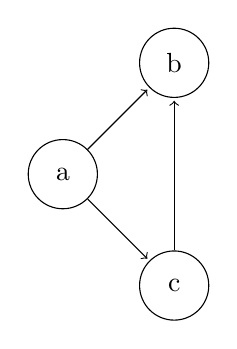
\begin{tikzpicture}[shorten >=1pt,node distance=2cm,on grid,auto] 
	\node[state] (a)   {a}; 
	\node[state] (b) [above right=of a] {b}; 
	\node[state] (c) [below right=of a] {c}; 
	\path[->] 
	(a) edge  node {} (b)
            edge  node {} (c)
	(c) edge  node {} (b)
            ;
\end{tikzpicture}\\
For the given graph above, V = \{a, b, c\}, E = \{(a, b), (a, c), (c, b)\}.\\
Let source vertex is a, $E_p$ = \{(a, c), (c, b)\} $\in$ E. Then $E_p$ cannot be produced by running BFS since edge 
(c, b) can be only produced when current vertex is c. However, b is already be visited as adjacent vertex of a. \\

Ref.\\
BFS, C. (2018). Creating simple path edges not contained in BFS. [online] Stack Overflow. Available at: https://stackoverflow.com/questions/5100991/creating-simple-path-edges-not-contained-in-bfs [Accessed 16 Jul. 2018].\\

% 6
6.\\
After dividing input elements into pairs, we need $\lfloor \frac{n}{2} \rfloor$ comparisons for all the pairs. 
So there are $\lceil \frac{n}{2} \rceil$ elements in all the pairs that is possible to be the maximum, 
and $\lceil \frac{n}{2} \rceil$ elements in all the pairs that is possible to be the minimum.\\
In order to get both maximum and minimum, $(\lceil \frac{n}{2} \rceil -1) * 2$ comparisons are necessary.
So, in the worst case, comparisons count $T(n) >= \lfloor \frac{n}{2} \rfloor + \lceil \frac{n}{2} \rceil - 1 + \lceil \frac{n}{2} \rceil - 1$.\\
Since $\lfloor \frac{n}{2} \rfloor + \lceil \frac{n}{2} \rceil = n$ and n is an integer.\\
So $T(n) >= n - 1 + \lceil \frac{n}{2} \rceil - 1 = \lceil \frac{3n}{2} \rceil - 2$.\\


\end{document}
